\section{Algorithm design} \label{sec:algorithm-design}

\fxnote{Hele introen her skal laves om. Det er tydelig copy paste. Antag at NN er den bedste, men grundet hardware testen skal NIV vælges i stedet. Tilføj lidt traveling salesman}

In order to solve the problem described in \secref{sec:problem-description}, a heuristic is needed. Since it is not f

%After the \projname{} has completed its initial 360 degree search and stored the information about the nearby objects, it is time to calculate a route between said objects. Due to the limited power and calculation speed of the LEGO NXT brick it is necessary to find an efficient algorithm that is fast and does not take a lot of computational power and space, in addition to finding a short route to all the objects. 

%After all the objects have been spotted, using the 360 degree search, an intelligent route to pick up these objects is needed. As mentioned in \secref{sec:problem-description}, the problem the \projname{} is dealing with is a form of the ``travelling salesman problem''. In order to solve this problem, the algorithm ``Nearest neighbour''(NN) algorithm is used. 

%Another way to solve the problem is by using a ``Next-in-view'' algorithm, that rely on a constant update from the sensors. Moving until the sensors detects something relevant. 


\subsection{Nearest neighbour algorithm} \label{sec:nn-algorithm}
The NN-algorithm starts by doing a 360 degrees turn while scanning the area around it for objects. The distance and angle for each object are saved and when the robot is done scanning, a route will be calculated using trigonometry and the concepts from the NN-algorithm. These calculations will result in an array of instructions containing distances and angles. Each instruction will take the robot from the current position to the next object in sequence. The robot repeats the entire process if it didn't collect all of the objects.

The algorithm uses trigonometry to select the next object, by using the objects positions observed from the starting position. The degrees the \projname{} must turn, in order to get to the same heading as the object, is saved as instructions, along with the distance that needs to be travelled in order to get to it. 

These instructions must then be followed after the route has been calculated. \figref{fig:object_navigation_first} shows a situation where all the objects have been spotted, and now the \projname{} must decide which object that should be collected first. At this point the shortest object is easy to conclude, as the distance to all objects, from the starting position, is already known, based on information from the ultrasonic sensor. The shortest distance overall is found, and the object associated to this is remembered, and marked as collected, to remove this from consideration when finding the next objects. Another set of instructions is used to ensure that the \projname{} is pointing back, at the starting position. This is used to ease the calculations of the following objects. 

\begin{figure}[H]
     \center{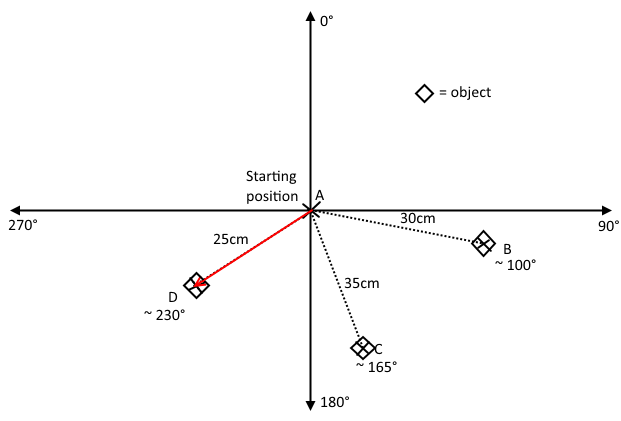
\includegraphics[width=\textwidth]
     {graphics/objectnavigationfirst.png}}
     \caption{\label{fig:object_navigation_first} First object to be collected.}
\end{figure}

Now that the first object has been scheduled to be collected, the NN-algorithm uses trigonometry to find the shortest distance to the next object, and calculates the angles that is needed to turn, to face the next object. To increase the understanding, the state of the world is represented in \figref{fig:object_navigation_iteration}, where the actions to collect the first object has been applied and reflected in the figure. From this point, the distance to the remaining objects is calculated, using the formula:
\begin{equation}
a = \sqrt{ b^2 + c^2 - 2*b*c*cos(A) } \label{equation:a}
\end{equation}

But for this, the A angle is needed. This is calculated from the spotted angles during the search. The formula for calculating A is:
\begin{equation}
A = (Object~currently~at~spotted~angle) - (Object~closest~spotted~angle) \label{equation:AAngle}
\end{equation}

With the same method as the first object, the object with the shortest distance, from the current object, is found and saves the object number. Now the heading to the closest object must be calculated, and this is the angle calculated by the formula:
\begin{equation}
B = cos^{-1}((a^2 + c^2 - b^2)/(2*a*c)) \label{equation:B}
\end{equation}

This provides the angle that must be turned in order to face the next object. In \figref{fig:object_navigation_iteration} the \projname{} is pointed towards the starting position, and the angle that must be turned is calculated from equation \ref{equation:B}. The current heading added with the angle provides the heading to the next object. This angle is added to the instructions along with the distance. Then the final angle of the triangle is calculated, which is used to turn the \projname{} at the starting position again. The final angle is calculated with the formula:
\begin{equation}
C = 180 - A - B \label{equation:C}
\end{equation}

In order to point the \projname{} at the starting position again, the current heading is subtracted with (180 - C), where C is found by equation \ref{equation:C}. This process has provided the route to the next object, and the instructions to turn the \projname{} back, facing the starting position. The second step is executed for the remaining objects that were spotted. 

\begin{figure}[H]
     \center{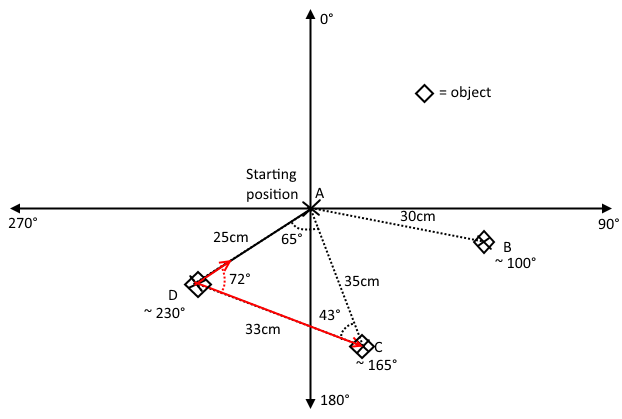
\includegraphics[width=\textwidth]
     {graphics/objectnavigationiteration.png}}
     \caption{\label{fig:object_navigation_iteration} Iteration of objects to be collected.}
\end{figure}


\subsection{Next-in-view algorithm} \label{sec:niv-algorithm}
An important property of the Next-in-view algorithm, is that it does not do any calculations prior to moving for objects, like the NN-algorithm. However it still relies a lot on the ultrasonic sensor, but in a different way. Instead of using the ultrasonic sensor to map the objects during the initial scan until all objects has been found, it uses the inputs from the sensor until all objects have been collected.

\begin{figure}[H]
     \center{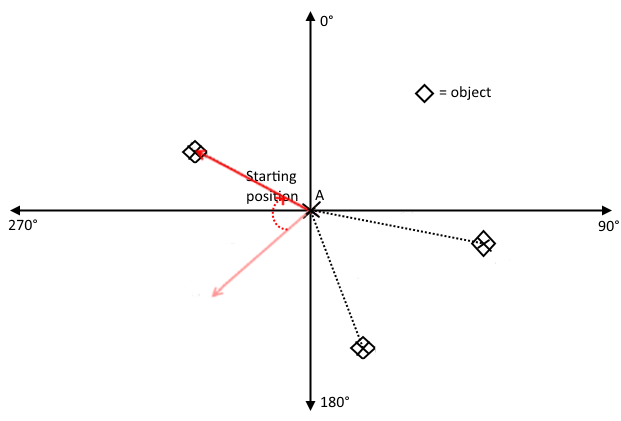
\includegraphics[width=\textwidth]
     {graphics/objectnavigationniv.png}}
     \caption{\label{fig:object_navigation_niv} Start-up using the Next-in-view algorithm}
\end{figure}

At start-up the robot starts turning until it spots an object with the sonar, as seen in \figref{fig:object_navigation_niv}. It then drives towards it until the object is within grabbing distance of the claw. The object will be picked up and the \projname{} continues to search for objects, as seen in \figref{fig:object_navigation_niv2}

\begin{figure}[H]
     \center{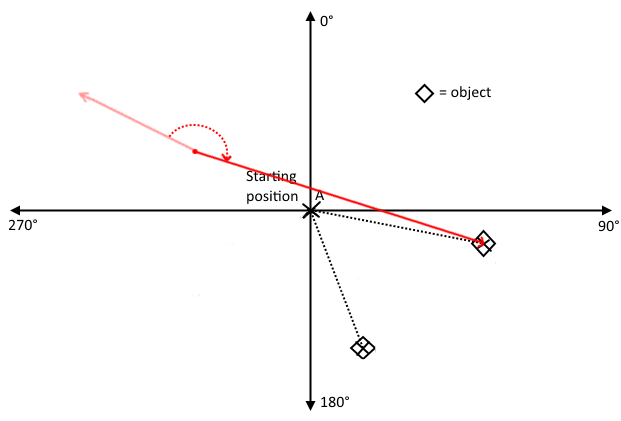
\includegraphics[width=\textwidth]
     {graphics/objectnavigationniv2.png}}
     \caption{\label{fig:object_navigation_niv2} Searching for the next object}
\end{figure} 

Because the ultrasonic sensors view is a cone, as described in \secref{sec:hardware}, a case may arise where the robot is not driving straight towards the object. But as it gets closer, it might lose the object as it gets out of the view of the sensor.

In this case, a small routine will be initiated, where the robot will turn a little to the right, followed by a little to the left, constantly scanning for objects, while slowly increasing the angles turned to scan an increasingly larger range. When an object is spotted again, the robot continues to move towards it. When the object has been collected, the robot starts turning until it finds a new object and the entire process continues until every object has been found.


\subsection{Algorithm comparison} \label{sec:algorithm-desc}

The shortest route between the object can be brute forced by trying out every single possible route between the start position and all of the objects.  This would have a calculation time of $\mathcal{O}(n!)$, which means that every object added, the running time greatly increases. This gives the robot problems when calculating a shortest route, if the amount of objects exceed a certain number, due to its limited processor power. If there are 9 objects for instance, the number of different paths to check exceeds 360000. This is an example of the traveling salesman problem as described in \secref{sec:problem-description}.

A faster, but less distance-efficient algorithm is the NN-algorithm. The algorithm calculates a route based on which objects are closest together. This means that the distance to all the points are calculated from the starting point and the shortest distance is chosen. This is then repeated from the new point, but this time it does not include the objects from previously visited points.

An algorithm that doesn't spend time on calculations prior to moving for objects is the next-in-view algorithm. This algorithm has a number of issues connected to it, which may reduce its performance, however in smaller cases with less than ten objects, its completion speed is close to the NN-algorithm.

\begin{figure}[H]
     \center{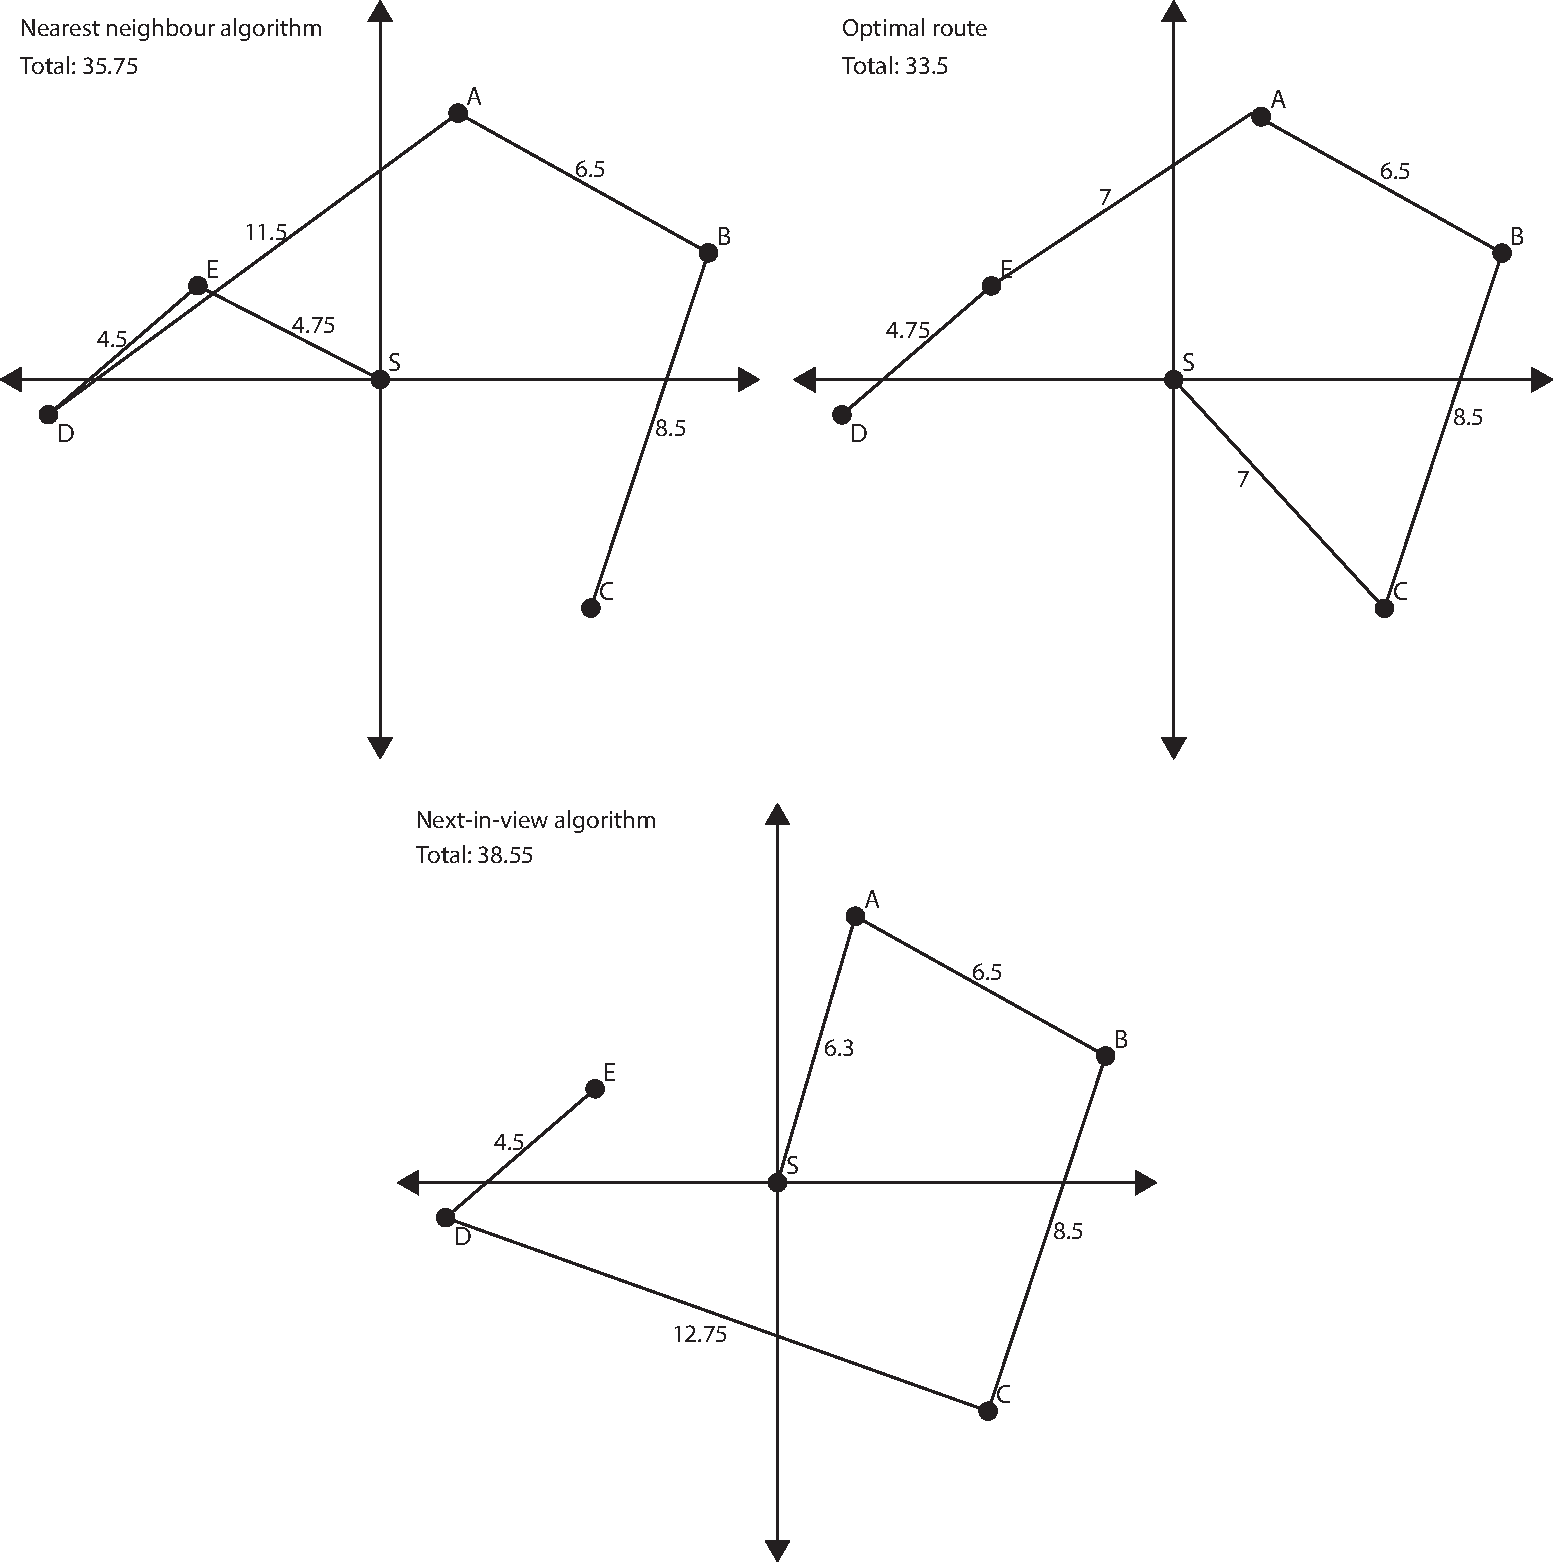
\includegraphics[width=\textwidth]
     {graphics/AlgorithmExamples2.pdf}}
     \caption{\label{fig:algorithm-example} Example of the NN-algorithm, the optimal algorithm, and next-in-view algorithms.}
\end{figure}

\figref{fig:algorithm-example} shows three solutions to the problem. The top right graph is the optimal solution, which is only used to compare the results from the two other algorithms. Top left is the NN-algorithm, and in the bottom the next-in-view algorithm. The robot starts its route at position \emph{S}. The objects are named in order as they are first detected. The algorithms result in the routes shown on the figure.

The different solutions in \figref{fig:algorithm-example} have following lengths:
\begin{itemize}
\item Optimal: 33.5 units
\item NN-algorithm: 35.75 units
\item Next-in-view: 38.55 units
\end{itemize}

In the average case, the difference between the NN-algorithm and the next-in-view solutions would be larger if there were more objects to consider. However for these smaller cases, the difference is almost negligible. It should be noted, that this does not describe the time spent, only the distance travelled: rotation to scan for objects, for both algorithms, will also take different amounts of time depending on the case. This is not accounted for here.

Due to the limitations of the LEGO NXT brick and the complexity of the problem, finding the optimal solution was ruled out as a possibility. Instead, the NN-algorithm was initially selected to calculate the route for the \projname{}. This algorithm does not always result in the most optimal route, but when the calculation speed and actual running speed is considered, it is arguably faster in the average case. 

As a result of this and the inaccurate hardware, it is chosen not to implement the NN-algorithm in the final version. The ultrasonic sensor was not able to detect objects with enough precision, that the \projname{} could accurately calculate any useful information based on the data. Due to this limitation, the \emph{next-in-view} algorithm was chosen for implementation. As mentioned in test case from \secref{sec:nn-algorithm} were the difference between the two algorithms' distance nearly insignificant. This also means that using a state-based representation of the world is preferred, where each state represents the robots behaviour. If the NN-algorithm were used, a feature based representation would be better suited for the \projname{}, because of the need to map the location of each found object in relation to the environment.
